%%%%%%%%%%%%%%%%%%%%%%%%%%%%%%%%%%%%%%%%%
% Memo
% LaTeX Template
% Version 1.0 (30/12/13)
%
% This template has been downloaded from:
% http://www.LaTeXTemplates.com
%
% Original author:
% Rob Oakes (http://www.oak-tree.us) with modifications by:
% Vel (vel@latextemplates.com)
%
% License:
% CC BY-NC-SA 3.0 (http://creativecommons.org/licenses/by-nc-sa/3.0/)
%
%%%%%%%%%%%%%%%%%%%%%%%%%%%%%%%%%%%%%%%%%

\documentclass[letterpaper,11pt]{texMemo} % Set the paper size (letterpaper, a4paper, etc) and font size (10pt, 11pt or 12pt)

\usepackage{parskip} % Adds spacing between paragraphs
\usepackage[colorlinks]{hyperref}
\usepackage{graphicx}
\usepackage{float}
\usepackage{listings}
\hypersetup{citecolor=DeepPink4}
\hypersetup{linkcolor=red}
\hypersetup{urlcolor=blue}
\usepackage{cleveref}
\setlength{\parindent}{15pt} % Indent paragraphs

%----------------------------------------------------------------------------------------
%	MEMO INFORMATION
%----------------------------------------------------------------------------------------

\memoto{Dr.Randy Hoover} % Recipient(s)

\memofrom{Benjamin Lebrun, Benjamin Garcia} % Sender(s)

\memosubject{Lab Assignment 4: Remote Control} % Memo subject

\memodate{\today} % Date, set to \today for automatically printing todays date

%\logo{\includegraphics[width=0.1\textwidth]{logo.png}} % Institution logo at the top right of the memo, comment out this line for no logo

%----------------------------------------------------------------------------------------

\begin{document}

\maketitle % Print the memo header information

%----------------------------------------------------------------------------------------
%	MEMO CONTENT
%----------------------------------------------------------------------------------------

\section*{Introduction}
%This section \textit{briefly} communicates what you have been asked to accomplish in the lab, how you approached it, and what results you saw. This is \textbf{not} an area for manifestos.

This project required us to create a console application that would read whether a pin was connected to a 5-volt source (would read 'high') or was not (would read 'low'). The application was also required to allow setting other pins to output high/low and to drive LEDs. The console portion was required to output an appropriate error message if invalid inputs were provided. The types of invalid inputs that could be detected included invalid commands (those other than 'set' or 'read'), invalid pins (set operations were only valid for pins 8 and 10, while read operations were only valid for pins 9 and 11), and invalid states (anything other than 'high' or 'low').

We began by creating an input interrupt handler, a buffer for input, and a stream object for output. This allowed us to read input from the interrupt handler into the buffer, and to output information back to the console using the stream object. Once basic IO was handled, we wrote code to tokenize the input on spaces and check the inputs for validity. If input was valid, the appropriate state values were set and execution continued. If input was invalid, the state flags would be set to error values and an appropriate message would be output. Once input processing was finished, low-level IO functions would be invoked based on the command and pin specified, and read or write operations with the pins were performed. After all processing and reading/writing, a message indicating the result of the command is printed to the terminal, and the program awaits further input.

Physically, we use push-buttons connected to the breadboard to handle reading high or low values from pins 9 and 11. If the button is pressed, the pins read 'high' as they are connected to the 5-volt source on the board, otherwise they read low. We have attached LEDs to the buttons to provide a visible indication of when the pins should read 'high' or 'low'.

On reset, the output pins start low, and the input pins are pulled low by the internal pull-down resistors. This means that the LEDs begin off and the read pins are 'low' before any user input is performed. When pin 8 is set high by the 'set 8 high' command, our blue LED will turn on. Similarly, when pin 10 is set high, the red LED will turn on. If either is set low by the 'set (8|10) low" command, the respective LED will turn off. The read pins (9 and 11) read low until their respective buttons are pushed. When the button for pin 9 is pressed, the yellow LED will turn on, and a read from the pin will report 'high'. Similarly, when the button for pin 11 is pressed, the green LED will turn on, and a read on pin 11 will report 'high'.


\section*{Equipment}
This lab required the following equipment:
\begin{itemize}
\item 4 resistors (220$\Omega$)
\item 4 LEDs
\item 2 push-buttons
\item 8 wires (male-male)
\item 1 USB-A to USB-B cable
\item 1 breadboard
\item 1 Arduino UNO (ATMega328P)
\item AVR 8-bit GCC toolchain
\item Putty
\end{itemize}

\subsection*{Configuration}
% TODO describe in words the circuit

\begin{figure}[!ht]
\begin{center}
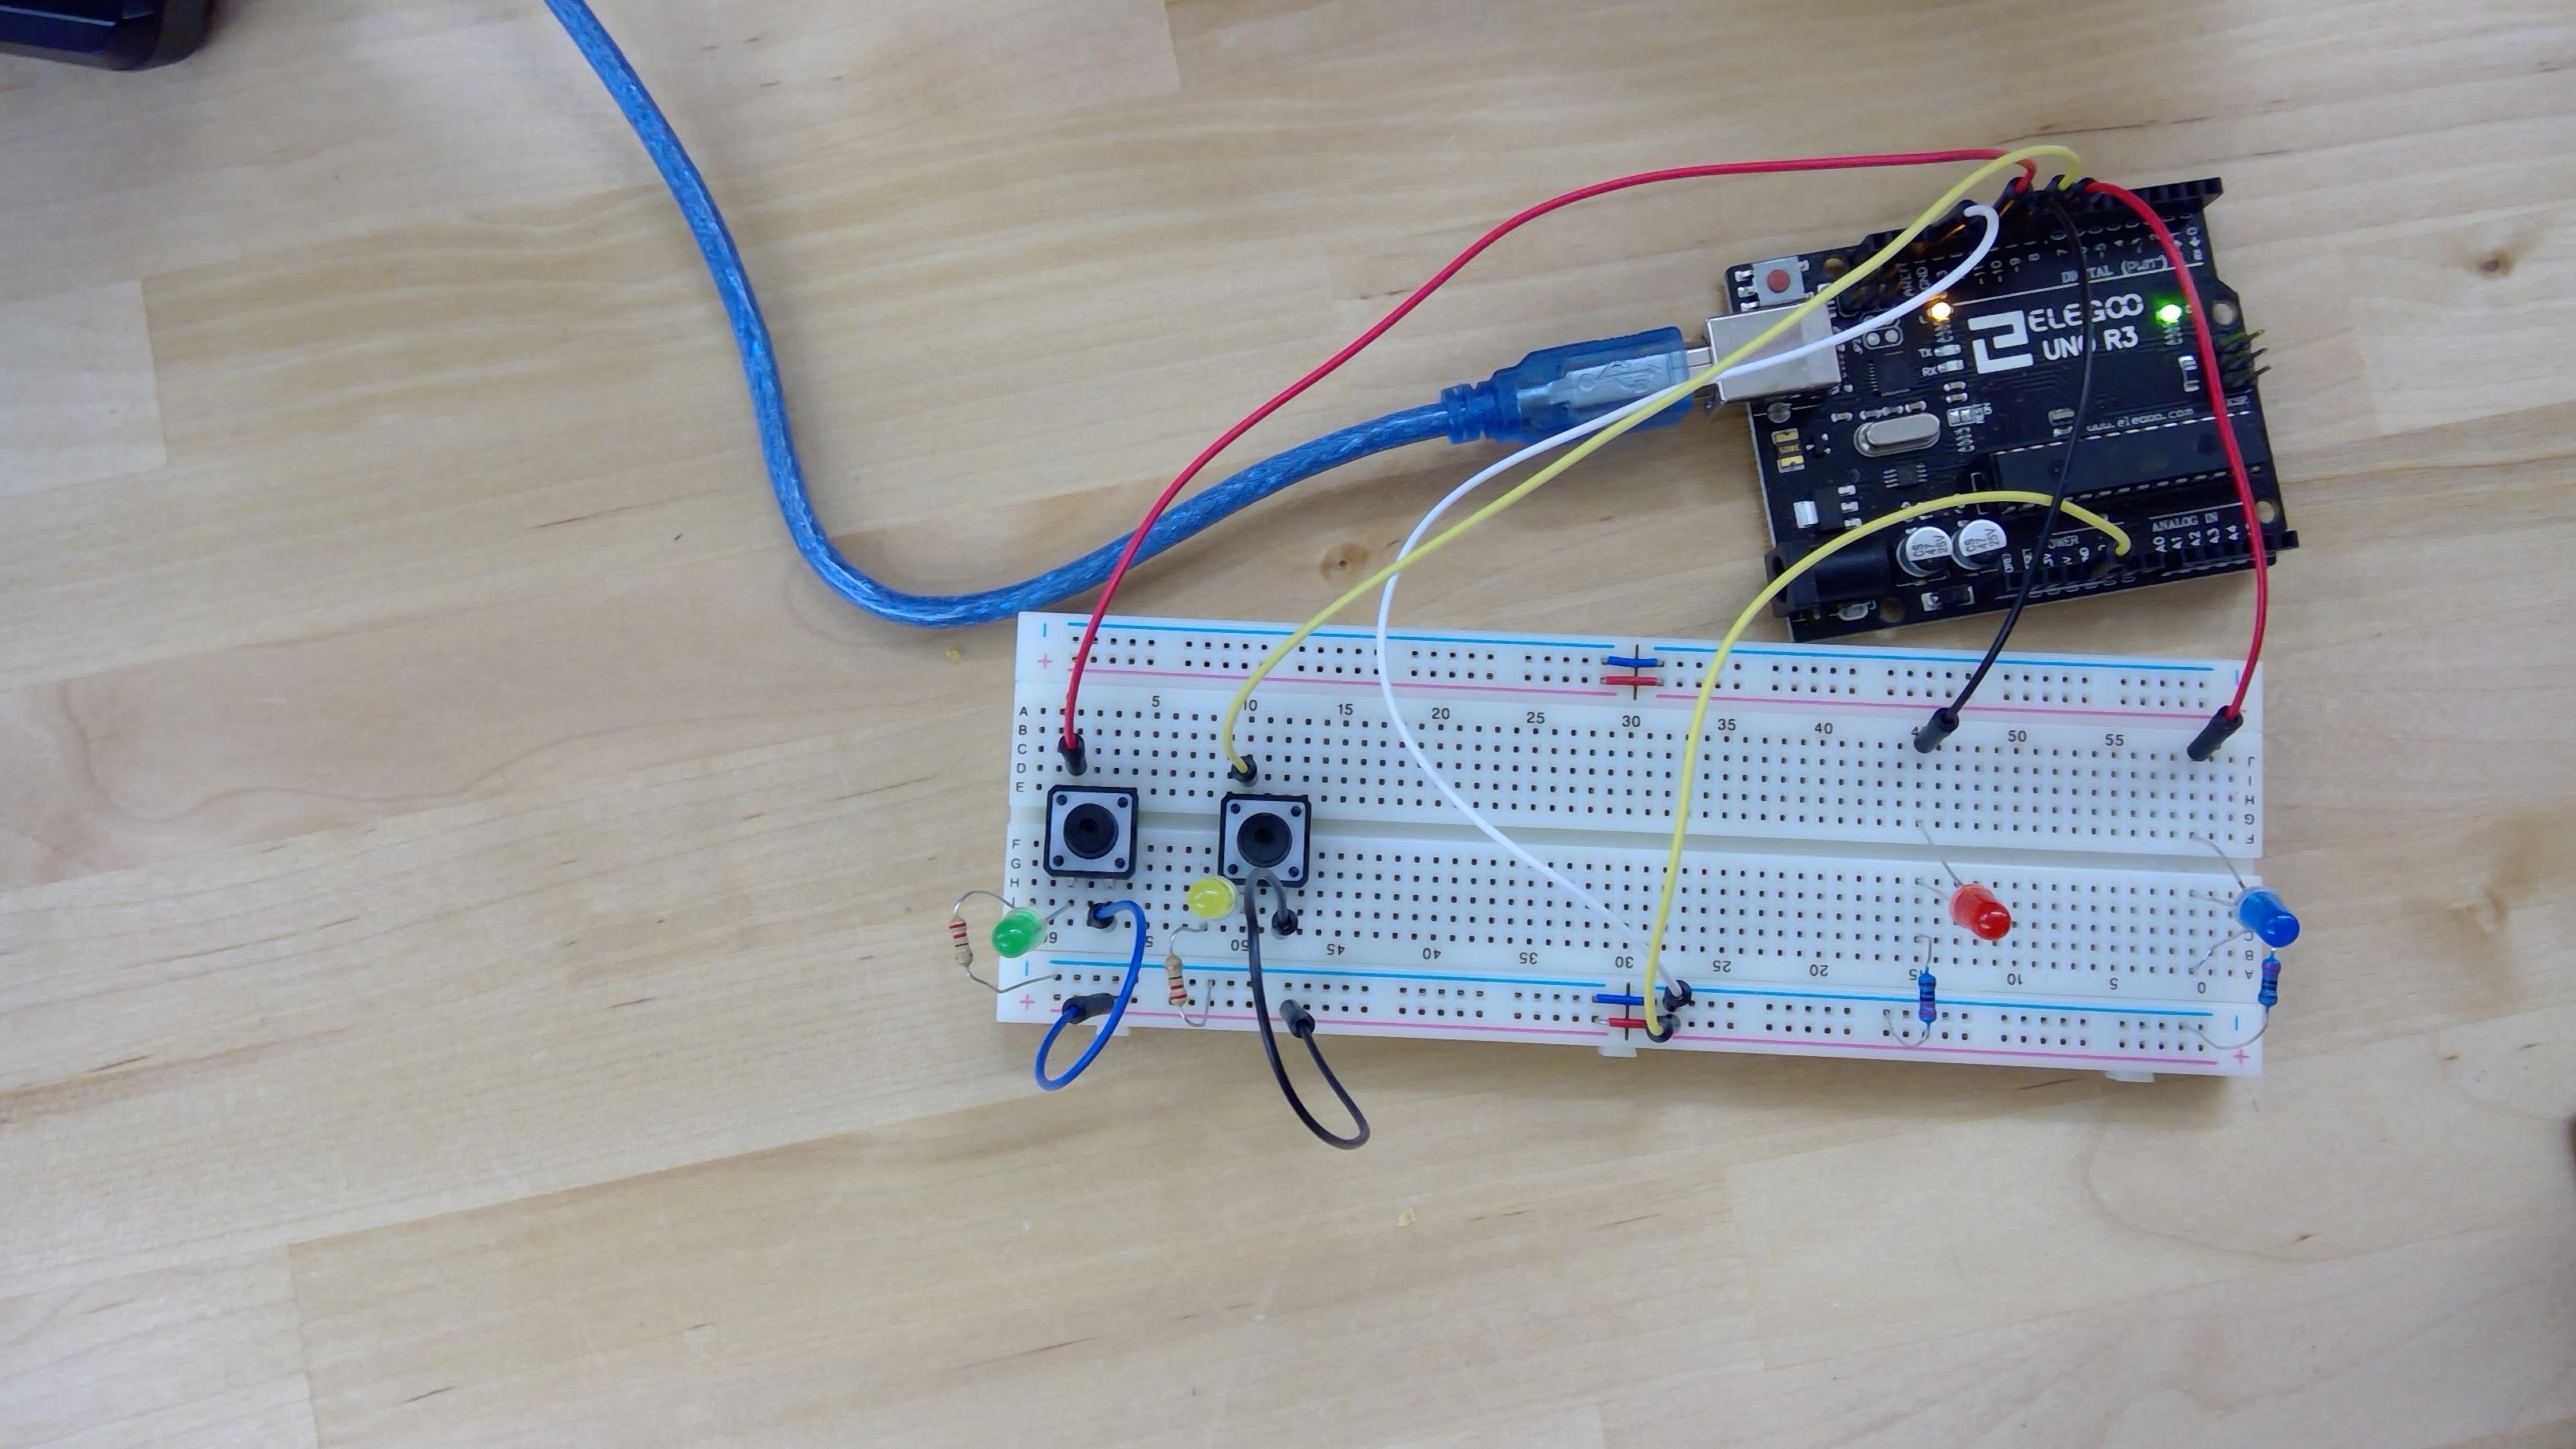
\includegraphics[width=\linewidth]{./configuration.jpg}
\caption{Picture of the wiring setup}
\end{center}
\end{figure}

\newpage
\section*{Implementation}

\subsection*{int main(void)}
%TODO
\subsection*{void setMessageType(char iobuff[])}
%TODO
\subsection*{void setPinNumber(char iobuff[], enum MSG_TYPE mode)}
%TODO
\subsection*{setPinMode(char iobuff[])}
%TODO
\subsection*{processMessage(char iobuff[])}
%TODO
\subsection*{ISR(USART_RX_vect) (interrupt)}
%TODO
\subsection*{void initUART()}
%TODO
\subsection*{void printMsg}
%TODO
\subsection*{static int uart_putchar(char c, FILE* stream)}
%TODO
\subsection*{enum MSG_TYPE}
%TODO
\subsection*{enum TGT_PIN}
%TODO
\subsection*{enum SET_TYPE}
%TODO
\subsection*{enum INVALID_TYPE}
%TODO
\subsection*{void initPins()}
%TODO
\subsection*{int ReadPinDigital(enum TGT_PIN pin}
%TODO
\subsection*{int WritePinDigital(enum TGT_PIN pin, enum SET_TYPE mode}
%TODO
\subsection*{strings.h}
%TODO

\section*{Discussion}


\newpage
\section*{Responses}


\section*{Appendices}
The following files are included as appendices:
\begin{itemize}
\item main.c - entry file, manages initialization logic.
\end{itemize}
\newpage

\section*{Appendix A: main.c}
\begin{tiny}
\lstinputlisting{../main.c}
\end{tiny}
\newpage
\end{document}
